%# -*- coding: utf-8 -*-
% !TEX encoding = UTF-8 Unicode
\RequirePackage{fixltx2e}
\documentclass[aps,pre,12pt,preprint,onecolumn,showpacs,showkeys,UTF8]{revtex4-1}
\usepackage{ctex}
\usepackage{mathrsfs}
\usepackage{setspace,dcolumn}
\usepackage{subfigure}
\usepackage{graphicx,psfrag,epsfig}
\usepackage[font=small,format=plain,labelfont=bf,textfont=it,justification=raggedright,singlelinecheck=false]{caption}
\usepackage{amsmath,amsfonts,amssymb,amsthm,bm,upgreek}
\usepackage{geometry}
\usepackage[mathscr]{eucal}
\usepackage{titlesec}
\usepackage{tabularx}
\titleformat{\section}{\bf\fangsong\zihao{4}}{\thesection}{0.75em}{}
\geometry{top=2.54cm,bottom=2.54cm,left=3cm,right=3cm}
\renewcommand\appendixname{附录}
\renewcommand\abstractname{}%摘要
\renewcommand\tablename{表}
\renewcommand\figurename{图}
\makeatletter
\def\@keys@name{\songti\zihao{-4}{\bf 关键词:}}
\def\Received@name{\zihao{-5}{接收} }
\def\Revised@name{\zihao{-5}{修订} }
\def\Accepted@name{\zihao{-5}{采纳} }
\def\Published@name{\zihao{-4}{发表} }
\makeatother
\linespread{1.6}
\renewcommand{\labelenumi}{\alph{enumi}.}
\leftmargini=20mm

\begin{document}

\title{\bf\heiti\zihao{3}体效应器的工作特性和波导管的工作状态\vspace{15mm}}
\author{\fangsong 乔颢\vspace{2mm}}
\affiliation{\songti\zihao{-4}北京大学物理学院2011级2班~~~~学号:1100011354 \vspace{2mm}}
\keywords{体效应振荡器,微波}
\email{1993422qsh@gmail.com; 18600200672}
\begin{abstract} 
	\vspace{10mm}
	\begin{spacing}{1.5}
		\songti\zihao{-4}本实验测量得到了体效应器的工作特性和电压之间的关系。并且测量了波导管中微波的驻波比和反射比。由次试验得到光速为光速为$c=3.002\times10^8m/s$。而微波的相速度为$v_g=\lambda_g f = 4.546\times 10^8m/s$,群速度为$u = 1.982 \times 10^8 m/s$。同时可以得到检波率n=1.804。

	\end{spacing}
\end{abstract}

\maketitle

\section{引言}

微波是波长很短,频率很高的电磁波。因为他的一系列特殊性质使得他在国防、通信、生产、科学研究等等方面有着广泛的应用。而了解微波的产生和传输的特性,掌握一些关键的基本参数,对于熟悉掌握微波技术是必不可少的。

微波的产生往往是用一些特殊的微波电子管产生。本实验中使用的是体效应振荡器,他体积小,结构简单,使用方便。其原理主要是利用Gunn效应,当加载n-GaAs样品上的电压超过一个临界阈值的时候,其会形成高场畴从而产生一个周期的电流振荡。产生的电流振荡的频率与样品的长度成反比。与畴的移动速度成正比。将体效应样品放在适当的谐振腔中,便会产生微波振荡。

微波一般会在波导管中传播。其中往往存在着入射波和反射波。描述波导管中匹配和反射程度的物理量是驻波比或反射系数。当波导管的工作状态是陪陪状态时,不存在反射波。驻波状态时,终端发生全反射,混波状态则是部分反射。在波导管中传播的微波,其相速度可以高于光速,但是能量传播的速度群速度则是小于光速的。 三者满足以下关系。
\begin{equation}
	v_g u = x^2
\end{equation}

总结来说,通过本实验希望能够了解体效应振荡器的结构、工作原理和工作特性以及波导管的三种工作状态。掌握微波的三种基本参数的测量方法等。

\section{实验仪器和过程}
实验装置如图所示:
\begin{figure}[h]
	\begin{center}
		\includegraphics[width=0.7\textwidth]{pic1.png}
		\caption{\label{g:1}微波实验线路图}
	\end{center}
\end{figure}

微波信号由固态源提供,整个设备工作在3cm波段。主要原件有隔离器、衰减器、吸收式频率机、驻波测量线和单螺调配器。

\subsection{体效应器的工作特性}

首先测量体效应器的工作特性。调整短路活塞和单螺调配器,使得检波输出电流合适。然后测量在不同电压下,工作电流,输出的微波功率等数据。得具体的数据如下:

\begin{table}[ht]
	\centering
	\begin{tabular}{m{3cm}<{\centering}m{3cm}<{\centering}m{3cm}<{\centering}m{3cm}<{\centering}}
		\hline
		\hline
		U/V	&	I/mA	&	f/GHz	&	P	\\
		\hline
8.00	&	306	&	8.614	&	10.5	\\
8.25	&	306	&	8.635	&	22.5	\\
8.50	&	305	&	8.651	&	38.5	\\
8.75	&	304	&	8.665	&	52.5	\\
9.00	&	303	&	8.676	&	76.0	\\
9.25	&	302	&	8.686	&	89.5	\\
9.50	&	302	&	8.695	&	98.5	\\
9.75	&	300	&	8.702	&	100.0	\\
10.00	&	300	&	8.710	&	100.0	\\
10.25	&	299	&	8.716	&	99.0	\\
10.49	&	298	&	8.721	&	96.5	\\
10.75	&	298	&	8.727	&	95.0	\\
11.00	&	297	&	8.732	&	93.0	\\
11.24	&	296	&	8.735	&	92.0	\\
11.49	&	296	&	8.739	&	90.5	\\
11.75	&	295	&	8.742	&	89.5	\\
11.99	&	295	&	8.745	&	89.0	\\
12.25	&	294	&	8.748	&	88.0	\\
12.49	&	294	&	8.750	&	88.0	\\
12.75	&	294	&	8.753	&	86.0	\\
12.95	&	298	&	8.756	&	85.0	\\
		\hline
	\end{tabular}
	\caption{体效应管的工作电流,输出频率,相对输出功率与电压之间的关系。(部分数据略)}
	\label{tab:table1}
\end{table}

从图表中可以看出,体效应管的工作电流在快速增加达到一个阈值之后基本稳定,输出频率随电压逐渐的增加,而输出的相对功率在迅速增加后达到最大值,然后逐渐的减少。

\begin{figure}[ht]
	\begin{center}
		\subfigure[]{
		\includegraphics[width=0.4\textwidth]{pic2.png}
		}
		\subfigure[]{
		\includegraphics[width=0.4\textwidth]{pic3.png}
		}
		\subfigure[]{
		\includegraphics[width=0.4\textwidth]{pic4.png}
		}

	\end{center}
	\caption{(a)体效应管工作电流和电压之间的关系图。(b)体效应管输出频率和电压之间的关系图。(c)体效应管输出功率和电压之间的关系图。}
	\label{fig:fig2}
\end{figure}

\subsection{微波在波导管的工作状态}

随后观察波导管的工作状态。调整输出频率显示为9GHz,实际频率$f=8.743GHz$。调整单螺调配器到最佳匹配状态,可以测量的道此时的驻波比。测量三次最大电流和最小电流关系可以得到:
\begin{equation}
	\rho = \frac{|E_{max}|}{|E_{min}|} = 1.028
\end{equation}
此时的反射系数为:
\begin{equation}
	|\Gamma_0|=(\rho - 1)/(\rho + 1) = 0.014
\end{equation}

同样的可以测量混波状态的驻波比和反射系数,调整到混波状态得到 $\rho = 2.26$, $|\Gamma_0|=0.386$。

接下来则是测量波导波长,读书电流计为10的位置,可以得到两个极小点之间的间距为$\lambda_g=52.0mm$。 此时的频率为$f=8.742GHz$。所以可以计算得到:
\begin{equation}
	\lambda=\frac{\lambda_g}{\sqrt{1+(\frac{\lambda_g}{2a})^2}}=0.03434m
\end{equation}
由此可以计算得到光速为$c=3.002\times10^8m/s$,相速度为$v_g=\lambda_g f = 4.546\times 10^8m/s$,群速度为$u = 1.982 \times 10^8 m/s$。

\subsection{驻波曲线}

测量得到驻波的曲线如下:
\begin{table}[ht]
	\centering
	\begin{tabular}{m{3cm}<{\centering}m{3cm}<{\centering}m{3cm}<{\centering}m{3cm}<{\centering}}
		\hline
		\hline
l/mm	&	I	&	l/mm	&	l	\\
\hline
102.8	&	0.0	&	117.0	&	107.5	\\
104.0	&	4.0	&	118.0	&	101.0	\\
105.0	&	11.0	&	119.0	&	93.0	\\
106.0	&	21.0	&	120.0	&	83.5	\\
107.0	&	31.5	&	121.0	&	72.0	\\
108.0	&	44.0	&	122.0	&	60.0	\\
109.0	&	57.5	&	123.0	&	46.5	\\
110.0	&	71.5	&	124.0	&	33.0	\\
111.0	&	84.0	&	125.0	&	21.0	\\
112.0	&	94.0	&	126.0	&	12.0	\\
113.0	&	102.5	&	127.0	&	5.5	\\
114.0	&	108.0	&	128.0	&	1.0	\\
115.0	&	111.0	&	129.0	&	0.5	\\
116.0	&	110.5	&	130.0	&	4.0	\\
\hline
	\end{tabular}
	\caption{微波在波导管里传播的驻波数据}
	\label{tab:table1}
\end{table}

根据终端距离l计算可以得到某一点的电场大小,可以做出电流I和电场强度的相对关系图,如下所示:

\begin{figure}[ht]
	\begin{center}
		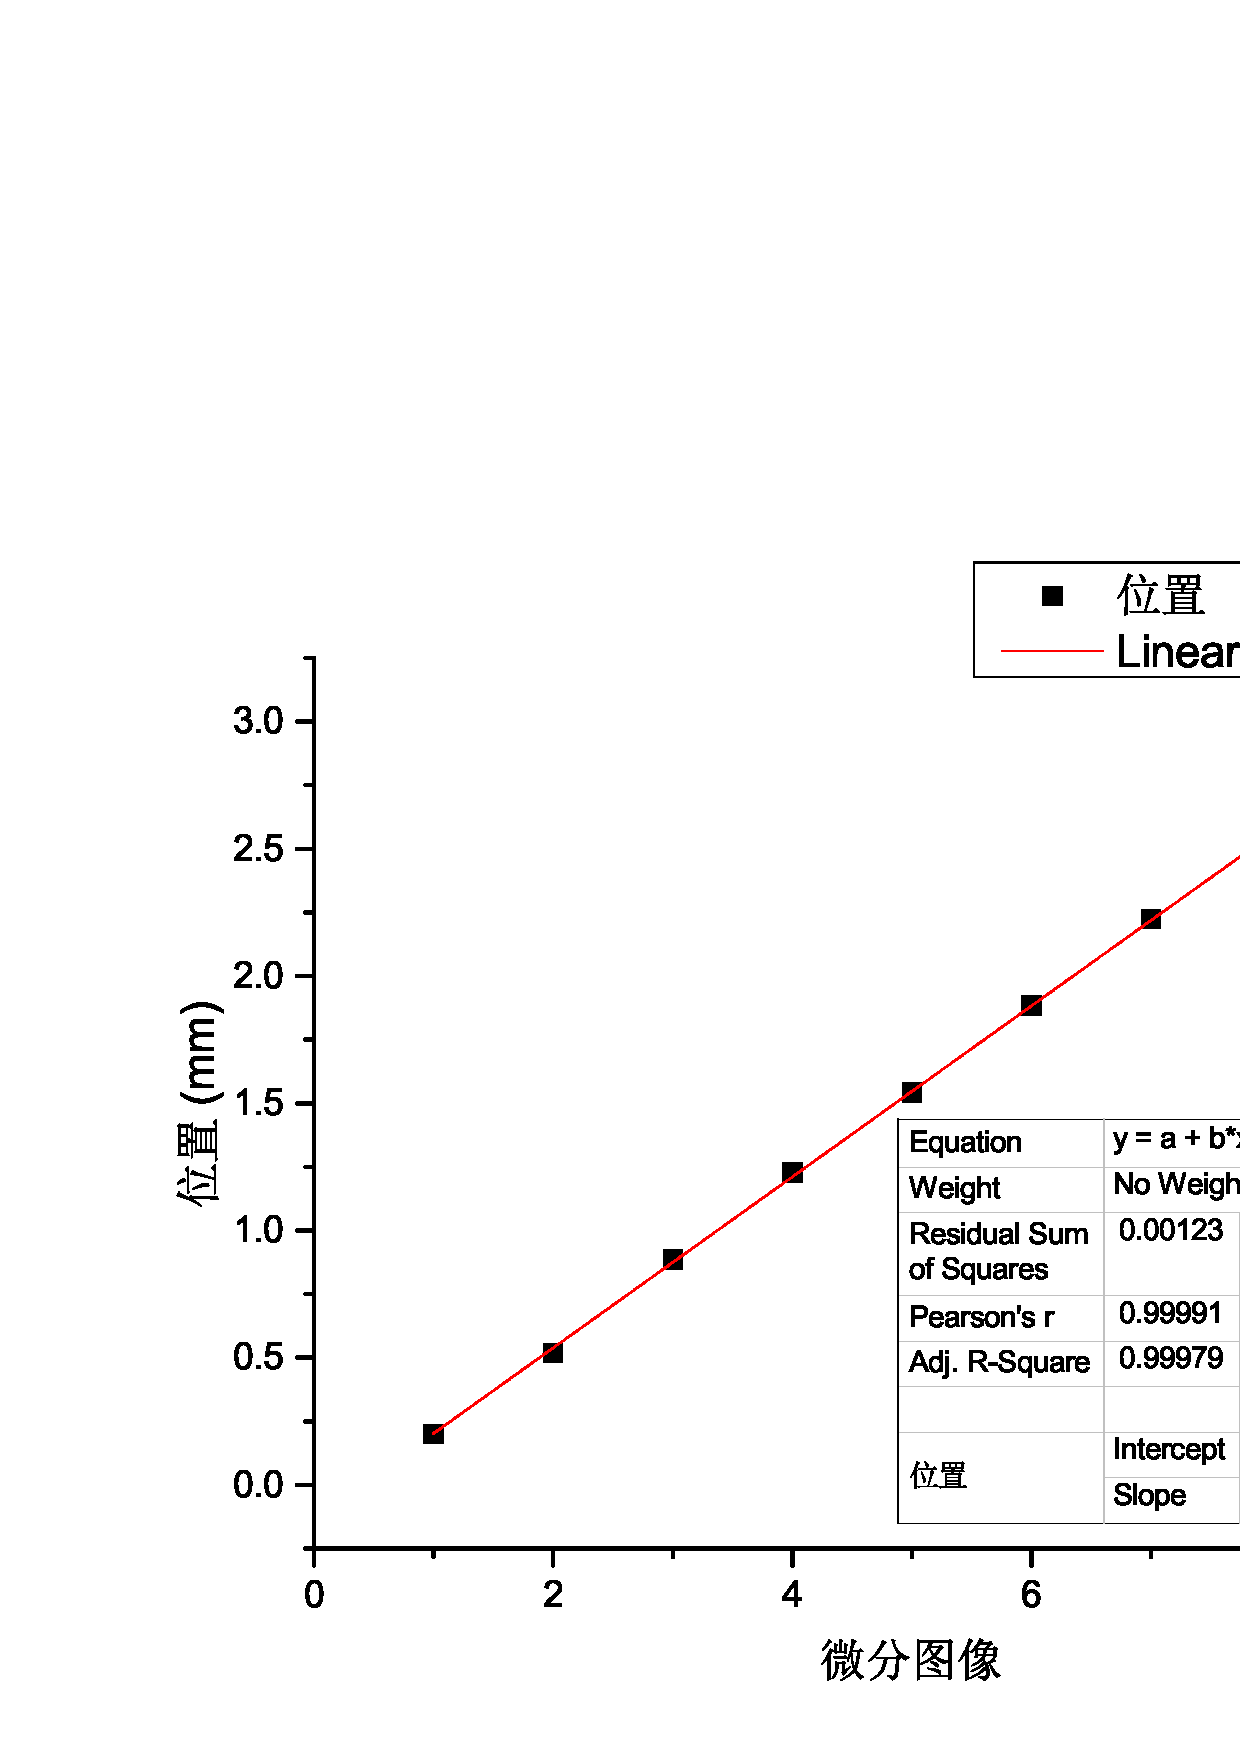
\includegraphics[width=0.7\textwidth]{pic6.png}
	\end{center}
	\caption{检波晶体管的电流和电场的关系图。}
	\label{fig:fig2}
\end{figure}

可以看出得到图曲线的两部分的重合性并不是特别的好,更有点像是有一点相位差或者说畸变。也就是说电流和距离之间的关系的对称性不是特别的好。这一点原因并不知道是什么,可能是因为边界条件等因素。

绘制检波管电流和距离之间的关系图可以计算得到n,数据图如下:
\begin{figure}[ht]
	\begin{center}
		\includegraphics[width=0.7\textwidth]{pic5.png}
	\end{center}
	\caption{检波晶体管的电流和位置的关系图。}
	\label{fig:fig2}
\end{figure}
可以得到半高宽为13.6mm, 从而计算得到n = 1.804。

\section{结论}

体效应管样品在长度一定的情况下,工作电流随着工作电压增加而增加,达到阈值后基本保持稳定。输出频率随着电压增加而增加,而输出功率也是在增加到一个阈值后慢慢减少。

波导管中微波的相速度为$v_g=\lambda_g f = 4.546\times 10^8m/s$,群速度为$u = 1.982 \times 10^8 m/s$。此时检波率n=1.804。

\section{致谢} 
感谢杜红林老师的指导,以及贾春燕,冉书能老师的技术支持。

\begin{thebibliography}{}
	\bibitem{Book} 吴思成,王祖铨~2010 近代物理实验(第三版)(北京:高等教育出版社)第165页.%
%
\end{thebibliography}

\clearpage
\appendix
\section{思考题} 

5cm波波长超过波导管的长端,所以不能传播。3cm可以传播,因为3cm大于波导管的短端而小于长端,所以可以传播TE10波。2cm则可以传播TE10和TE01。

\end{document} 
